\section{Immagini}
Un'immagine a colori viene percepita dal sistema visivo grazie all'impatto con le onde elettromagnetiche, caratterizzate dalla lunghezza d'onda $\lambda$ (proporzionale all'inverso della frequenza, $\lambda \propto \frac{1}{v}$) e dall'ampiezza (intensità). La lughezza d'onda è rapportata il periodo: indica quanto ci mette un ciclo a compiersi.

Lo spettro è in buona parte invisibile, con estremi alti che corrispondono alle radiazioni ultraviolette e bassi a radiazioni infrarosse. La porzione visibile è misurata in nanometri, con ordini di grandezza molto alti.

\begin{figure}[h]
	\centering
	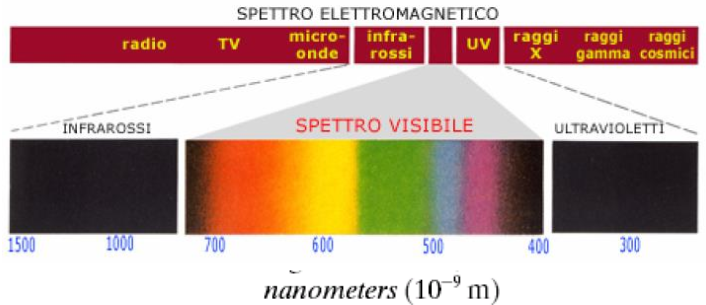
\includegraphics[scale=0.6]{Lezioni/Immagini/arcobaleno}
\end{figure}

Il cristallino focalizza l'immagine sulla retina come una lente, e il colore è processato nella retina da coni e bastoncelli, in numerose tipologie con risposte differenti a seconda della lunghezza d'onda. Essi convertono le onde elettromagnetiche in uno stimolo elettrico.

I coni producono segnale per livelli di luminosità più alti, e possono essere:
\begin{itemize}
	\item L (long waves), sensibili al rosso;
	\item M (middle waves), sensibili al verde;
	\item S (short waves), sensibili al blu.
\end{itemize}

I bastoncelli funzionano con le rappresentazioni in toni di grigio, esono in percentuale estremamente maggiore; essendo essi atti a misurare la variazione d'intensità, gli esseri umani hanno più sensibilità in condizioni di scarsa luce. La percezione ultima del colore è legata a intensità e crominanza (tinta, saturazione), e le due dimensioni sono separabili. 

L'occhio è più sensibile alle variazioni di luce nel centro dello spettro visibile, quindi lo spettro avrà la forma di una curva con funzione che varia al variare delle lunghezze d'onda. A seconda dei nanometri della radiazione, alcuni coni saranno attivati, eventualmente fondendo le risposte: il colore è combinazione di contributi a diverse lunghezze (spettro).

\begin{figure}[h]
	\centering
	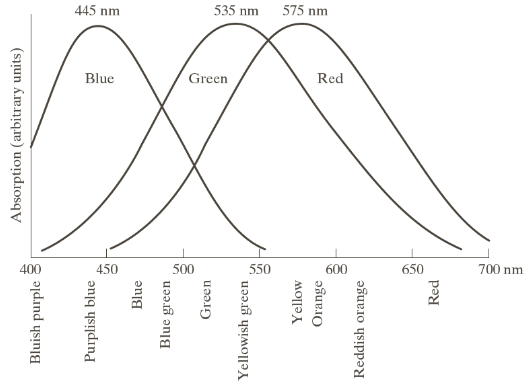
\includegraphics[scale=0.6]{Lezioni/Immagini/coni}
\end{figure}

\subsection{Segnale reale}
Per descrivere esattamente il segnale che forma l'immagine a partire da una scena occorre:
\begin{itemize}
	\item $E(\lambda)$, distribuzione spettrale dell'illuminante (SPD);
	\item $R(\lambda)$, riflettanza spettrale di ogni elemento della scena;
	\item $S(\lambda)$, sensitività dei recettori (coni e bastoncelli).
\end{itemize}

L'oggetto assorbe una parte della radiazione e ne ritrasmette un'altra parte (parametri legati alla capacità di riflettere), i cui segnali interferiscono con i recettori umani. La luce visibile è quindi $E(\lambda) \cdot R(\lambda)$, e ogni colore può essere descritto da tre parametri (RGB).

La maggior parte delle sorgenti luminose produce contributi di luce su più lunghezze d'onda:
$$L = \int E(\lambda) R(\lambda) l(\lambda) d\lambda$$
$$M = \int E(\lambda) R(\lambda) m(\lambda) d\lambda$$
$$S = \int E(\lambda) R(\lambda) s(\lambda) d\lambda$$
I numeri in output si definiscono valori di stimolo, che poi si traducono nei canali RGB. Le distribuzioni continue in funzione di $\lambda$ si trasformano in valori discreti in spazio tridimensionale grazie all'integrale.

Le immagine acquisite da una fotocamera digitale sono differenti da quelle elaborate dall'occhio umano: il sistema visivo viene simulato tramite sensori e processamento. Ogni camera ha una matrice che trasforma il segnale in modo da renderlo simile all'output del cervello, e i valori ottenuti dai sensori sono interpolati. 

I dati sono fatti passare in filtri colore, disposti secondo Bayer pattern. Il verde è il colore recepito meglio, e permette di misurare maggiormente le variazioni di intensità (e conseguentemente i dettagli dell'immagine). 

\subsection{Sintesi}
La somma dei contributi delle onde è chiamata sintesi additiva, e viene usata dai dispositivi che imitano l'occhio umano; esiste anche la sintesi sottrattiva, che fa differenze in base allo spettro e ai colori complementari di RGB (ciano, magenta, giallo). 

Quest'ultima consiste nella sovrapposizione di più filtri: il colore che giunge alla vista è quello che riesce a passare per tutti i filtri, dato che ognuno di essi sottrae una parte della luce che lo attraversa. 

\begin{figure}[h]
	\centering
	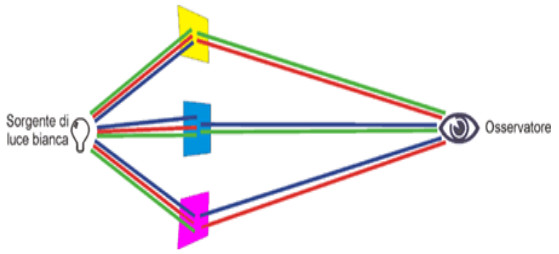
\includegraphics[scale=0.6]{Lezioni/Immagini/occhio}
\end{figure}


Esistono rappresentazioni che separano i canali in base alla loro intensità, mettendola in evidenza in base alla frequenza delle onde. Alcuni esempi di modelli sono:
\begin{itemize}
	\item RGB (red, green, blue), usato dalle camere e videocamere digitali;
	\item HSB (hue, saturation, brightness), corrisponde alla percezione umana del colore;
	\item HSV (hue, saturation, value), HSB con tinta definita su un angolo;
	\item CMYK (cyan, magenta, yellow, black), utilizzato per la sintesi sottrattiva nei sistemi di riproduzione;
	\item YIQ, per i segnali TV e VHS in America;
	\item YUV, per i segnali TV e VHS in Europa;
	\item YcbCr, per i video digitali.
\end{itemize}

Il formato grafico è la tecnologia utilizzata per memorizzare il file. Le immagini hanno due tipologie di formato: 
\begin{itemize}
	\item Raster, scalate in base a un numero prefissato di pixel e bit per pixel (bitmap) in una griglia di elementi, usate per digitalizzazione ed elaborazione di scene reali. L'accuratezza della rappresentazione dipende dal numero di pixel e dalla loro condifica (quantizzazione);
	\item Vettoriale, rappresentate con formule matematiche e oggetti, applicabili solo nel mondo geometrico ma con qualità maggiore. Le immagini sono più complesse e non viene persa definizione, ma sono più difficilmente modificabili.
\end{itemize}
Un'immagine in meta formato è una combinazione di questi formati, cioè contiene informazioni di ogni tipo: solitamente viene usato raster con alcuni elementi vettoriali.

\subsection{Risoluzione}
Le immagini hanno dimensioni espresse in pixel, mentre le dimensioni fisiche dipendono dal dispositivo di acquisizione. 

La risoluzione dà informazioni sulla quantità o la densità di pixel contenuti in un'immagine (ppi, pixel per inches). In caso di stampa o acquisizione con scanner si misura in dpi, dot per inches (gocce di inchiostro). Più alta è la risoluzione, più piccola è la dimensione fisica dei pixel: tipicamente una qualità alta di stampa ha una risoluzione intorno ai 300 ppi.

La risoluzione ottima dipende dallo scopo dell'immagine, tenendo conto di un fattore moltiplicativo di ingrandimento: esso rappresenta il rapporto tra il lato dell'immagine di destinazione e la sua dimensione fisica.

Esempio: diapositiva di $24\times36$ mm, da stampare in $10\times15$ in 300 ppi:
$$\frac{100\text{mm}}{24\text{mm}} \cdot 300\text{ppi} = 1248 \text{ppi}$$
Le immagini sugli schermi video solitamente sono acquisite in 72 dpi.
$$ \text{File size} = \frac{\text{height} \cdot \text{width} \cdot \text{bit depth} \cdot \text{dpi}}{8} = \frac{\text{pixel dimensions} \cdot \text{bit depth}}{8}$$

\subsection{Quantizzazione cromatica}
La profondità del colore è il numero di bit per pixel:
\begin{itemize}
	\item 1 bit rappresenta 2 colori (bianco e nero);
	\item 8 bit rappresentano 256 colori (colormap, livelli di grigio);
	\item 24 bit rappresentano quasi 17 milioni di colori (true color).
\end{itemize}

Per risparmiare sulla profondità si usano palette contenenti il sottoinsieme dei colori rappresentabili che compare in una foto. Una lookup table individua i corrispondenti valori di rosso, verde e blu.

Le dimensioni, la risoluzione e il numero di bit determinano l'occupazione in memoria, proporzionale a essi. Per una visualizzazione in scala $1 : 1$ l'immagine deve avere la stessa risoluzione del display.

Un istogramma rappresenta l'insieme dei valori che un segnale può assumere, espresso in livelli di quantizzazione. Non dà informazioni spaziali, ma solo sul contrasto e sul numero di bit: indica quanti campioni assumono un certo valore (quantizzatore ottimo), e in base a ciò è possibile decidere come applicare la compressione (probabilità normalizzata).

Il dynamic range è l'intervallo tra ampiezza massima e minima di un segnale, legato al numero di bit e al contrasto: se esso viene sfruttato appieno, l'immagine è ben contrastata. L'occhio umano può distinguere valori di luminosità massima/minima con un rapporto di circa $10.000 : 1$, mentre i monitor riproducono a $256 : 1$.

Per rappresentare meglio immagini con bianco o nero predominante, si utilizzano quantizzatori con pochi bit tagliando tutti i valori che non vengono utilizzati, in modo da avere una distribuzione più uniforme. 

L'occupazione del range dinamico dipende dal tempo di esposizione: più è breve, più la fotografia è luminosa. Il sistema HDR usa $n$ bit per catturare una porzione del range dinamico con differente esposizione, per poi sovrapporre tutte le immagini ottenute in modo da avere una visione più chiara. 

Per visualizzare scene con alto range dinamico (HDR) sui monitor, è necesario effettuare il tone mapping, cioè la riduzione in scala inferiore (8 bit). Il dithering è la conversione a una profondità colore inferiore: i pixel sono divisi in blocchi, ognuno dei quali viene riempito con diversi pattern di nero allo scopo di simulare i livelli di grigio. L'effetto è la perdita di risoluzione.

Per evitare i ``salti", ogi pixel è sostituito con un pattern più grande, in modo che il numero di punti stampati possa approssimare il livello di intensità (half tone printing). Le dimensioni, pertanto, sono più grandi. Per le immagini a colori, si usano vicinanze di colori diversi per crearn un altro osservando a distanza. 

Effettuando il dithering bisogna anche aggiungere rumore casuale: in questo modo le basse frequenze vengono nascoste dalle alte, e interferiscono con il rumore di quantizzazione ottenendo un disturbo più regolare e quindi percepito in misura minore.
